\begin{figure*}[ht]
\centering
\begin{minipage}[t]{0.3\textwidth}
    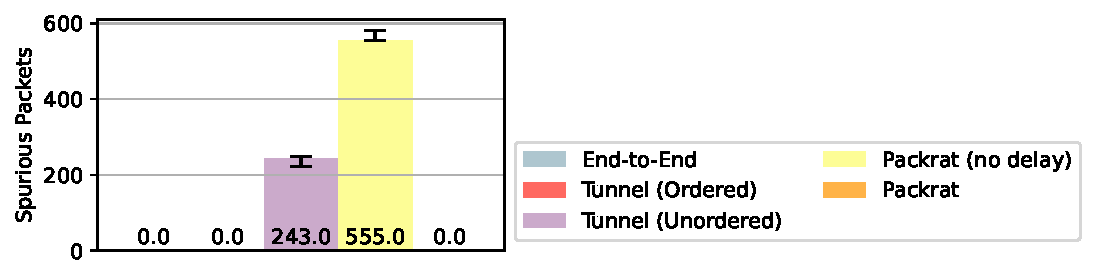
\includegraphics[width=\linewidth, trim=245 15 5 65, clip]{figures/spurious_retx_legend.pdf}
    \begin{subfigure}[b]{\linewidth}
        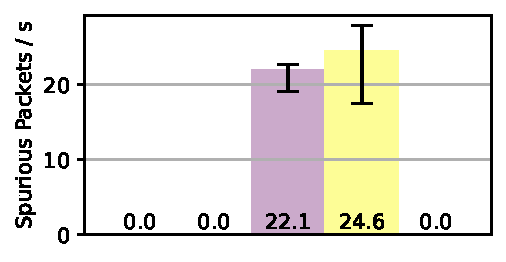
\includegraphics[width=\linewidth]{figures/spurious_retx_http.pdf}
        \caption{HTTP/3 download.}
        \label{fig:http:spurious}
    \end{subfigure}
    \begin{subfigure}[b]{\linewidth}
        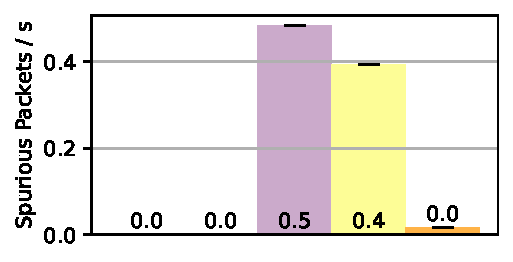
\includegraphics[width=\linewidth]{figures/spurious_retx_media.pdf}
        \caption{Low-latency media.}
        \label{fig:media:spurious}
    \end{subfigure}
    \caption{The unordered tunnel and \Sys without modifying the end-to-end reorder signal cause the client to receive spurious retransmissions. Modifying the end-to-end signal with \Sys significantly reduces them.}
    \label{fig:spurious}
\end{minipage}%
\hfill
\begin{minipage}[t]{0.68\textwidth}
    \centering
    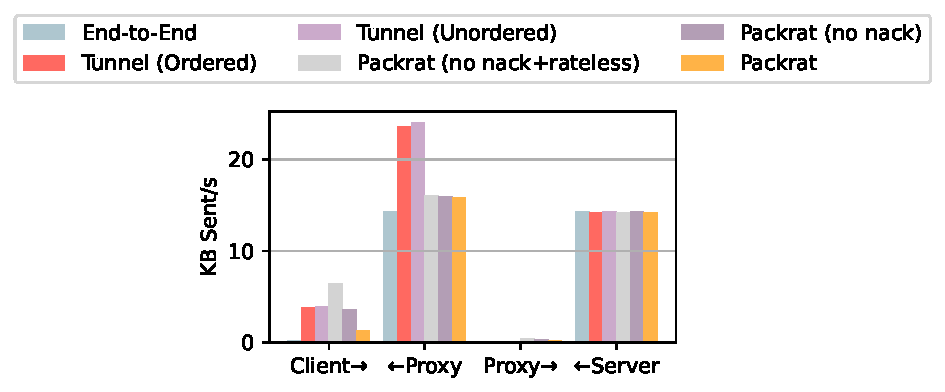
\includegraphics[width=0.9\linewidth, trim=5 140 5 5, clip]{figures/network_stats_media_legend.pdf}
    % 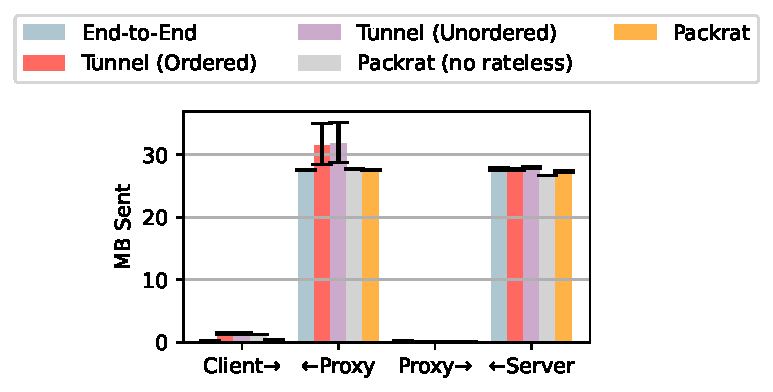
\includegraphics[width=0.7\linewidth, trim=5 140 5 5, clip]{figures/network_stats_http_legend.pdf}
    
    \begin{subfigure}[b]{0.48\linewidth}
        \centering
        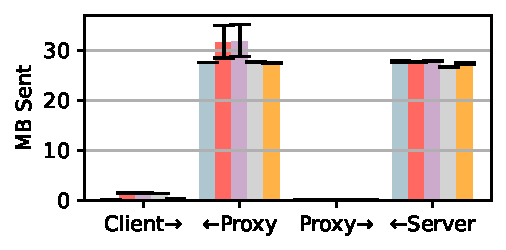
\includegraphics[width=\linewidth]{figures/network_stats_http_tx_bytes.pdf}
        \caption{HTTP/3 download (bytes).}
        \label{fig:link-overheads:http-bytes}
    \end{subfigure}
    \begin{subfigure}[b]{0.51\linewidth}
        \centering
        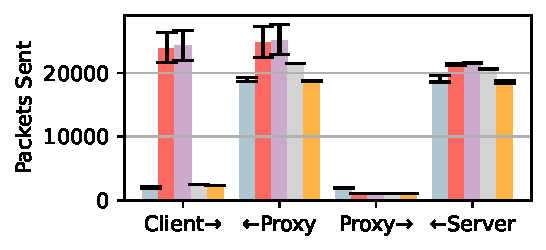
\includegraphics[width=\linewidth]{figures/network_stats_http_tx_packets.pdf}
        \caption{HTTP/3 download (packets).}
        \label{fig:link-overheads:http-packets}
    \end{subfigure}\\

    \begin{subfigure}[b]{0.49\linewidth}
        \centering
        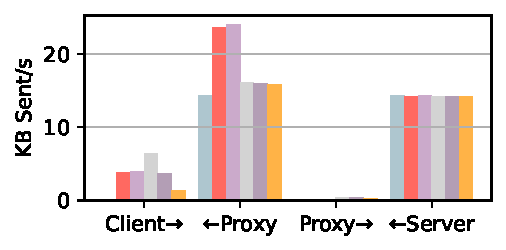
\includegraphics[width=\linewidth]{figures/network_stats_media_tx_bytes.pdf}
        \caption{Low-latency media (bytes).}
        \label{fig:link-overheads:media-bytes}
    \end{subfigure}
    \begin{subfigure}[b]{0.49\linewidth}
        \centering
        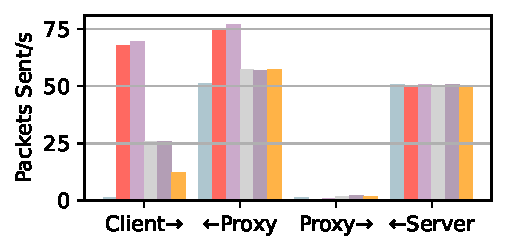
\includegraphics[width=\linewidth]{figures/network_stats_media_tx_packets.pdf}
        \caption{Low-latency media (packets).}
        \label{fig:link-overheads:media-packets}
    \end{subfigure}
    
    \caption{The number of bytes (left) and packets (right) sent between the
     client, proxy, and server. The statistics are captured directly from the
     network interface. The link overheads from eACKs in the \Sys protocol are
     comparable to those of the underlying acknowledgment scheme. The client
     sends fewer bytes with rateless eACKs, and fewer packets when it
     selectively eACKs. The tunnel aggressively ACKs and retransmits.}
    \label{fig:link-overheads}
\end{minipage}
\end{figure*}